% NetMed_McGarry.tex
% To be submitted to: Journal of Computational Biology and Chemistry
% https://www.journals.elsevier.com/computational-biology-and-chemistry/

\documentclass[authoryear,10pt,preprint]{elsarticle}
\usepackage{amssymb}
\usepackage{epsf}
\usepackage{graphicx}
\usepackage{epstopdf}
\usepackage{natbib} 
\usepackage{mathtools}
\usepackage[margin=1in]{geometry}
\usepackage{array}% http://ctan.org/pkg/array
\usepackage{amsmath} 
\usepackage{algorithmicx}
\usepackage{algorithm}
\usepackage{algpseudocode}
\usepackage{caption}
\usepackage{subcaption}
\usepackage{verbatim}

\begin{document}
\begin{frontmatter}
\title{Complex network medicine: exploration of disease and drug connectivity patterns through discovery of disease modules}

\author{Ken McGarry, Sharon McDonald and Jack Gallagher}
%\author[label2,label3]{Author2}
\address{School of Pharmacy and Pharmaceutical Sciences, \\University of Sunderland, City Campus, \\Sunderland, SR1 3SD, UK}

\begin{abstract}
In this work we use network science and graph theory to explore the dynamic nature of diseases, the genes implicated with them and the drugs used to treat them. We investigate the hypothesis that many human diseases or disorders are linked by common genetic modules, therefore a defect in one of any of the cooperating genes in a module may lead to a specific disease or related symptom. Furthermore, although faulty genes need not be directly shared between diseases they can interact with similar proteins in the network neighborhood. Thus, some diseases are indirectly linked and any analysis of disease genes must take this into account. We build our networks using data and information extracted from protein interaction databases, OMIM disease database, lists of diseases categorized by MeSH, the drugbank repository, along with supporting knowledge in the form of biological ontologies. We demonstrate how the complex network approach allows us to identify modules of cooperating proteins and ultimately, understand their role in disease with respect to targeting drugs more effectively. 
\end{abstract}

\begin{keyword}
Graph theory \sep networks \sep protein interactions \sep ontologies \sep diseasome
\end{keyword}

\end{frontmatter}

\section{Introduction}
Protein interactions are key to the majority of functions occurring in the cell and also account for several signaling mechanisms for processes external to the cell. The connectivity of interacting proteins ({\it interactome})  when mapped as a network reveals a complex web of relationships. Some proteins have many connections while others are sparsely connected, however applying computational techniques such as clustering can also reveal the modular nature of proteins as they cooperate in various activities \citep{Barabasi2011,McGarry2013}. Researchers have modified graph theoretic methods to tackle the issues inherent with protein interaction networks, or have implemented predicative algorithms for identifying protein function \citep{Nabieva05,Shafer06} and in particular identifying interesting sub-graphs using a combination of clustering and classification methods has received increased interest \citep{Lee11,Klamt06}. These computational techniques are essential to unraveling the complex nature of genes, proteins and their relationship with diseases. 

A high degree of heterogeneity exits both in genes and disorders, in particular some diseases are implicated with a small number of genes, while some medical problems such as colon cancer and deafness have been associated with more than thirty genes. However, most genes are generally associated with only a few diseases, on the other hand there are genes such as the tumor suppressor gene P53 which is known to be implicated with up to ten disorders. Clearly, these hub genes play an important role. Furthermore, diseases appear to be interlinked with the hub genes and can cause multiple problems when they become defective, the human disease network  or \emph{diseasome} \citep{Barrenas2009,McGarry2014a} is now receiving increased attention as a means of understanding how diseases occur. The objective is to develop novel drug products and to potentially reposition existing drugs to new targets \citep{He2011,Hu2009, McGarry2016a}. \citep{Menche2015,Ghiassian2015,Barabasi2011,Barabasi2004,Vidal2011}

Diseases can be classified according to their ICD10 (International Classification of Disease) codes and the MeSH (Medical Subject Headings) ontology. 

Recent observations confirm that a great degree of modularity occurs in protein networks with overlap or crosstalk of functionality \citep{McGarry2013,McGarry2014a}. This is likely to have arisen through evolution since it confers the benefits of robustness and the possibility of increasing the number of cellular functions with the same genetic machinery.  It may also lead to co-morbidity which implies the presence of one or more diseases in addition to the primary disease. The most often cited example of co-morbidity is the relationship between obesity and diabetes, where the structural changes in the adipose fatty tissues leads to an irreversible progressive defect in insulin secretion coupled with a progressive rise in insulin resistance. 

%%%%%%%%%%%%%%%%% Figure %%%%%%%%%%%%%%%%%
\begin{figure}[h]
%\epsfysize=4.0cm \leavevmode
  \begin{center}
 \includegraphics[width=12cm,height=8cm]{/Latex/DiseaseNets/systemDN2.pdf} % OK
  \end{center}
\special{center} \caption{Highly simplified disease network showing only three of the eight classes of Gastrointestinal diseases, each square node indicates a specific disease linked to the others by at least one shared protein. The C06 number is the level 2 MeSH code.}
\label{small_net}
\end{figure}
%%%%%%%%%%%%%%%%%%%%%%%%%%%%%%%%%%%%

Recent studies based on modeling cooperating modular groups of genes have suggested that diseases themselves are in fact network like \citep{BauerM2011,Barrenas2009}. The concept of the human disease network (HDN) or \emph{diseasome} is relatively new and is now starting to be explored as means of developing new drug products to tackle and combat diseases \citep{He2011,Hu2009}.  Figure \ref{small_net} shows only a small part of the connectivity relating to Gastrointestinal diseases. 

The view taken is that the diseasome is best represented as a bipartite graph formed by two sets of disjoint nodes, with the disease state forming one set and the other comprising the disease causing nodes \citep{GohKI2012}. The first network was constructed using data from the OMIM database and  links between the two sets of nodes were generated when mutations in a gene were implicated in a disorder\citep{Goh2007}.

%%%%%%%%%%%%%%%%% Figure %%%%%%%%%%%%%%%%
\begin{figure*}[ht]
%\epsfysize=4.0cm \leavevmode
  \begin{center}
 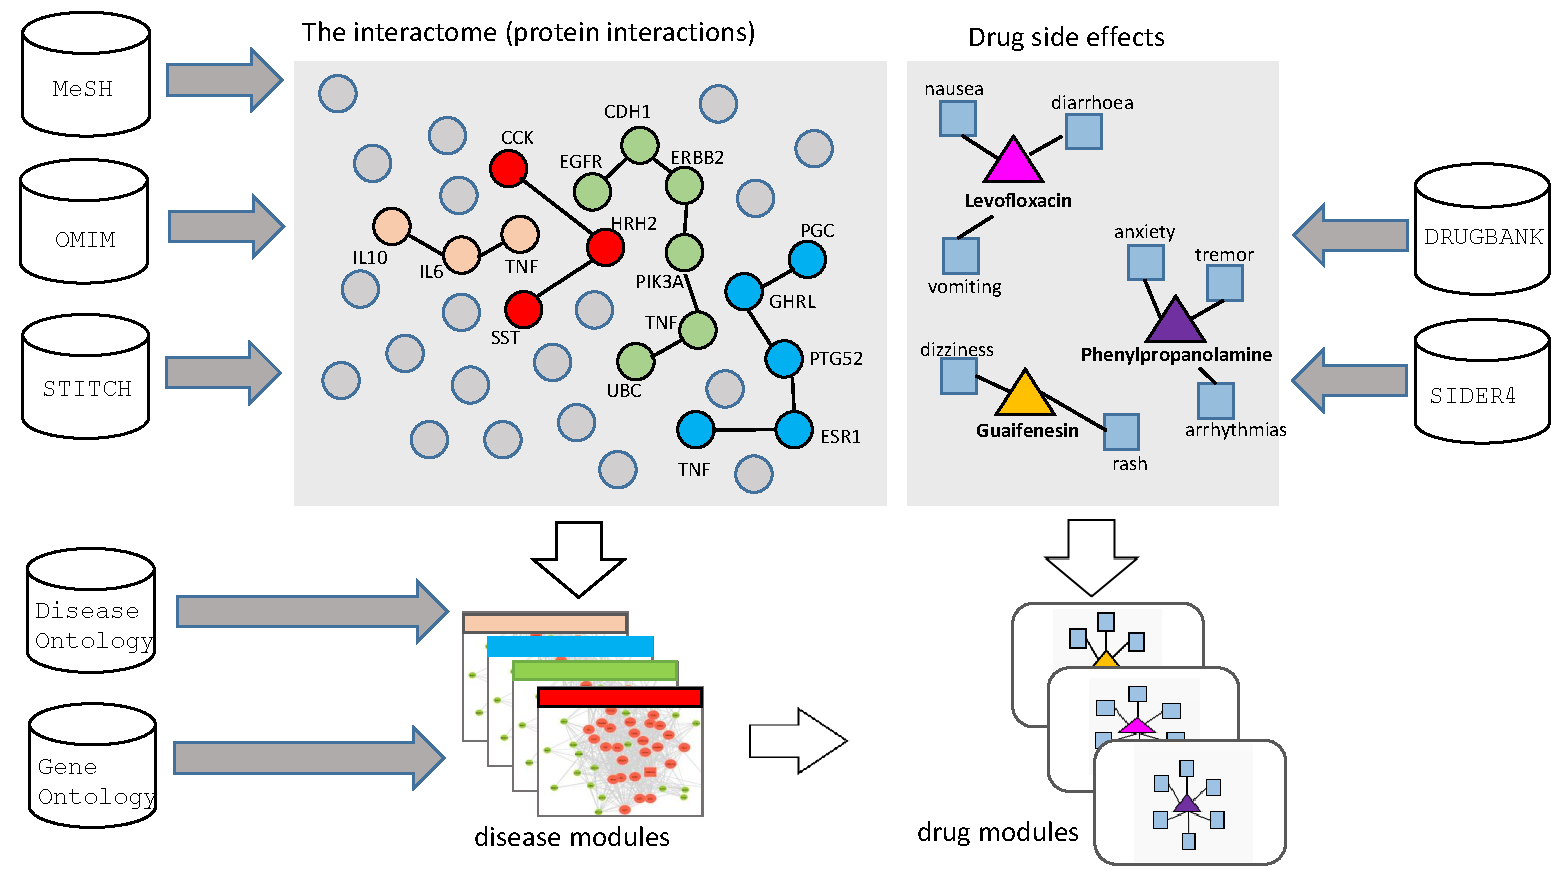
\includegraphics[width=15cm,height=10cm]{/LaTex/DiseaseNets/system_disease.pdf} % OK
  \end{center}
\special{center} \caption{The overall system operation, data sources and transformations.}
\label{system}
\end{figure*}
%%%%%%%%%%%%%%%%%%%%%%%%%%%%%%%%%%%%

There are many challenges to overcome when building accurate networks of disease,  most notably is the scale of the problem; the human genome consists of approximately 25,000 protein coding genes of which about 10\% have some linkage or association to a specific disease \citep{Barabasi2011}. Furthermore, there are approximately 1,000 known metabolites and chemicals that can interact with and modify the behavior of the protein products.  Additional complexity of the disease network comes in part from cooperating clusters of genes participating in more than one cellular function, loss of gene function can contribute to several disorders in humans. For example Zellweger syndrome, where long chains of fatty acids can accumulate in the tissues causing problems with the central nervous system has so far been linked to defects in any one of 11 genes \citep{Wanders04}. 

For other diseases, the issue however is not so straightforward as the other genes in a particular cluster may compensate for the malfunction of one gene, this is not so easy to identify \citep{LeePark2008}.  However, recent work has identified an underlying set of organizing principles that can be used to assess and identify the structures involved, we discuss these criteria in section two. A good overview of the technologies and challenges such as the cellular organization and the detection of structural motifs involved in network-based approaches to understanding diseases can be found in Barabasi \citep{Barabasi2004}.  

A number of challenges are presented by the nature of the data used in the construction of networks, most notably it breaks a number of statistical assumptions, for example there is a high degree of correlation within the cell of the metabolites and various activity patterns. This invalidates the important statistical assumption of independent variables. Also, the most powerful statistical techniques are parametric but the majority of proteomic data is highly skewed. Considering these limitations, our aim is to develop a computational model of the key aspects of the human disease network using graph mining and clustering. 

We can improve our knowledge and understanding of the mechanisms of disease and may suggest alternative therapeutic interventions \citep{McGarry2017a,McGarry2017b}. The remainder of this is paper is structured as follows; section two discusses the methods including the architecture of our system and the sources of data and knowledge; section three describes the experimental  results; section four presents the discussion and finally section five presents the conclusions and future work. 

\section{Related work}
Similar systems to ours have been developed such as the CIDeR network by Lechner et al \citep{Lechner2012}. The {DI}se{A}se {MO}dule {D}etection ({DIAMOnD}) algorithm by Ghiassian used a systematic analysis of connectivity patterns of disease proteins in the human interactome \citep{Ghiassian2015}. 

\section{Methods}
\subsection{Data and knowledge sources}
The chemical structure of the drugs was downloaded from the NCBI in SDFs (structure data files) format. These consist of a series of molfiles joined together, together with some further information about the compounds. They are frequently used for sharing libraries of compound structure data. \cite{Weininger1988}. We created a series of fingerprints for each drug based on atom-pair arrangements of 1024 bits in size which are stored in a matrix-like representation where every molecule is encoded as a fingerprint of the same type and length. The presence or absence of a particular structure is represented by a binary bit, either `1' or `0'. We consider the chemical structure of the drugs as useful information to assess their role in any disease network, and ultimately for drug repositioning.

%%%%%%%%%%%%%%%%% Figure %%%%%%%%%%%%%%%%
\begin{figure}[ht]
%\epsfysize=4.0cm \leavevmode
  \begin{center}              %angle=270,
    \  \includegraphics[width=4cm,totalheight=4cm]{/LaTex/DiseaseNets/SDF.jpg} % OK
  \end{center}
\special{center} \caption{SDF file format}
\label{sdf}
\end{figure}
%%%%%%%%%%%%%%%%%%%%%%%%%%%%%%%%%%%%



The candidate drugs have known on-target and off-target proteins, this knowledge is augmented by accessing protein-to-protein interactions and drug to protein interactions found in the STITCH and STRING databases \cite{Kuhn2012}. The STRING database  makes use of over six million known protein-to-protein interactions discovered by text mining and annotation by human experts. Additionally,  a further 30,000 associations are predicted based on similar protein characteristics using predictive data mining. The STITCH database contains protein to chemical mappings and augments the information held in Drugbank which may not contain all the potential drug to protein interactions. 

The Reactome database is accessed to provide indications of which biological pathways are involved with the on-target and off-target protein interactions affected by the candidate drugs \cite{Yu2015c}. Deeper insights can be gained into the biological functions by allowing users of the system to relate side-effects to drugs and then to the pathways. Individual proteins must not be regarded in isolation but seen as a system of interacting components. The associated pathways are incorporated into the overall drug ranking measure.


The system was implemented using the R language with the RStudio programming environment, on an Intel Xenon CPU, 64-bit with dual processors (3.2GHz) and 128 GB of RAM. The following R packages were used: BioassayR allows access to the PubChem database \citep{Backman2016}, other general purpose packages for data manipulation and complex network generation include; chemmineR, ggplot2, dplyr, tidyr, igraph, stringr.  Our R code and data files that generate the tables, diagrams and functional code described in this paper are freely available on GitHub for download: \\https://github.com/kenmcgarry/ComplexNetworkMedicine

\subsection{Using network theory to link diseases with genes}
Graph theoretic methods can be applied to any discipline where the entities of interest are linked together through various associations or relationships.  Quite diverse application areas such as social network analysis and biological networks are particularly suited to the mathematics of graph construction, traversal and inferencing.
A graph G = (V, E) consists of a set of nodes often called vertices V and a set of links called edges E, . The links in this case are undirected, that is to say there is no implied direction to the relationship in the sense that A causes B.

\begin{equation}\label{closeness}
     CC(v_i) =  \frac{N - 1}{\sum_{j} d(v_i,v_j)}
\end{equation}

The criteria we use to determine the relevance of disease connectivity is based upon recent discoveries.

It is likely that the essential genes and the disease genes encode the hubs.

\begin{itemize}
\item Topological module. Locally dense network of genes, often identified using clustering.
\item Functional module. Grouping of similar genes, where role is captured by function.
\item Disease module. Components that when damaged result in a particular disease or symptoms.
\end{itemize}


Recent observations confirm that a great degree of modularity occurs in protein networks with overlap or crosstalk of functionality. This is likely to have arisen through evolution since it confers the benefits of robustness and the possibility of increasing the number of cellular functions with the same genetic machinery.  It may also lead to co-morbidity which implies the presence of one or more diseases in addition to the primary disease. The most often cited example of co-morbidity is the relationship between obesity and diabetes, where the structural changes in the adipose fatty tissues leads to an irreversible progressive defect in insulin secretion coupled with a progressive rise in insulin resistance. 



\section{Results}


%%%%%%%%%%%%%%%%% Figure %%%%%%%%%%%%%%%%
\begin{figure*}[ht]
%\epsfysize=4.0cm \leavevmode
  \begin{center}              %angle=270,
    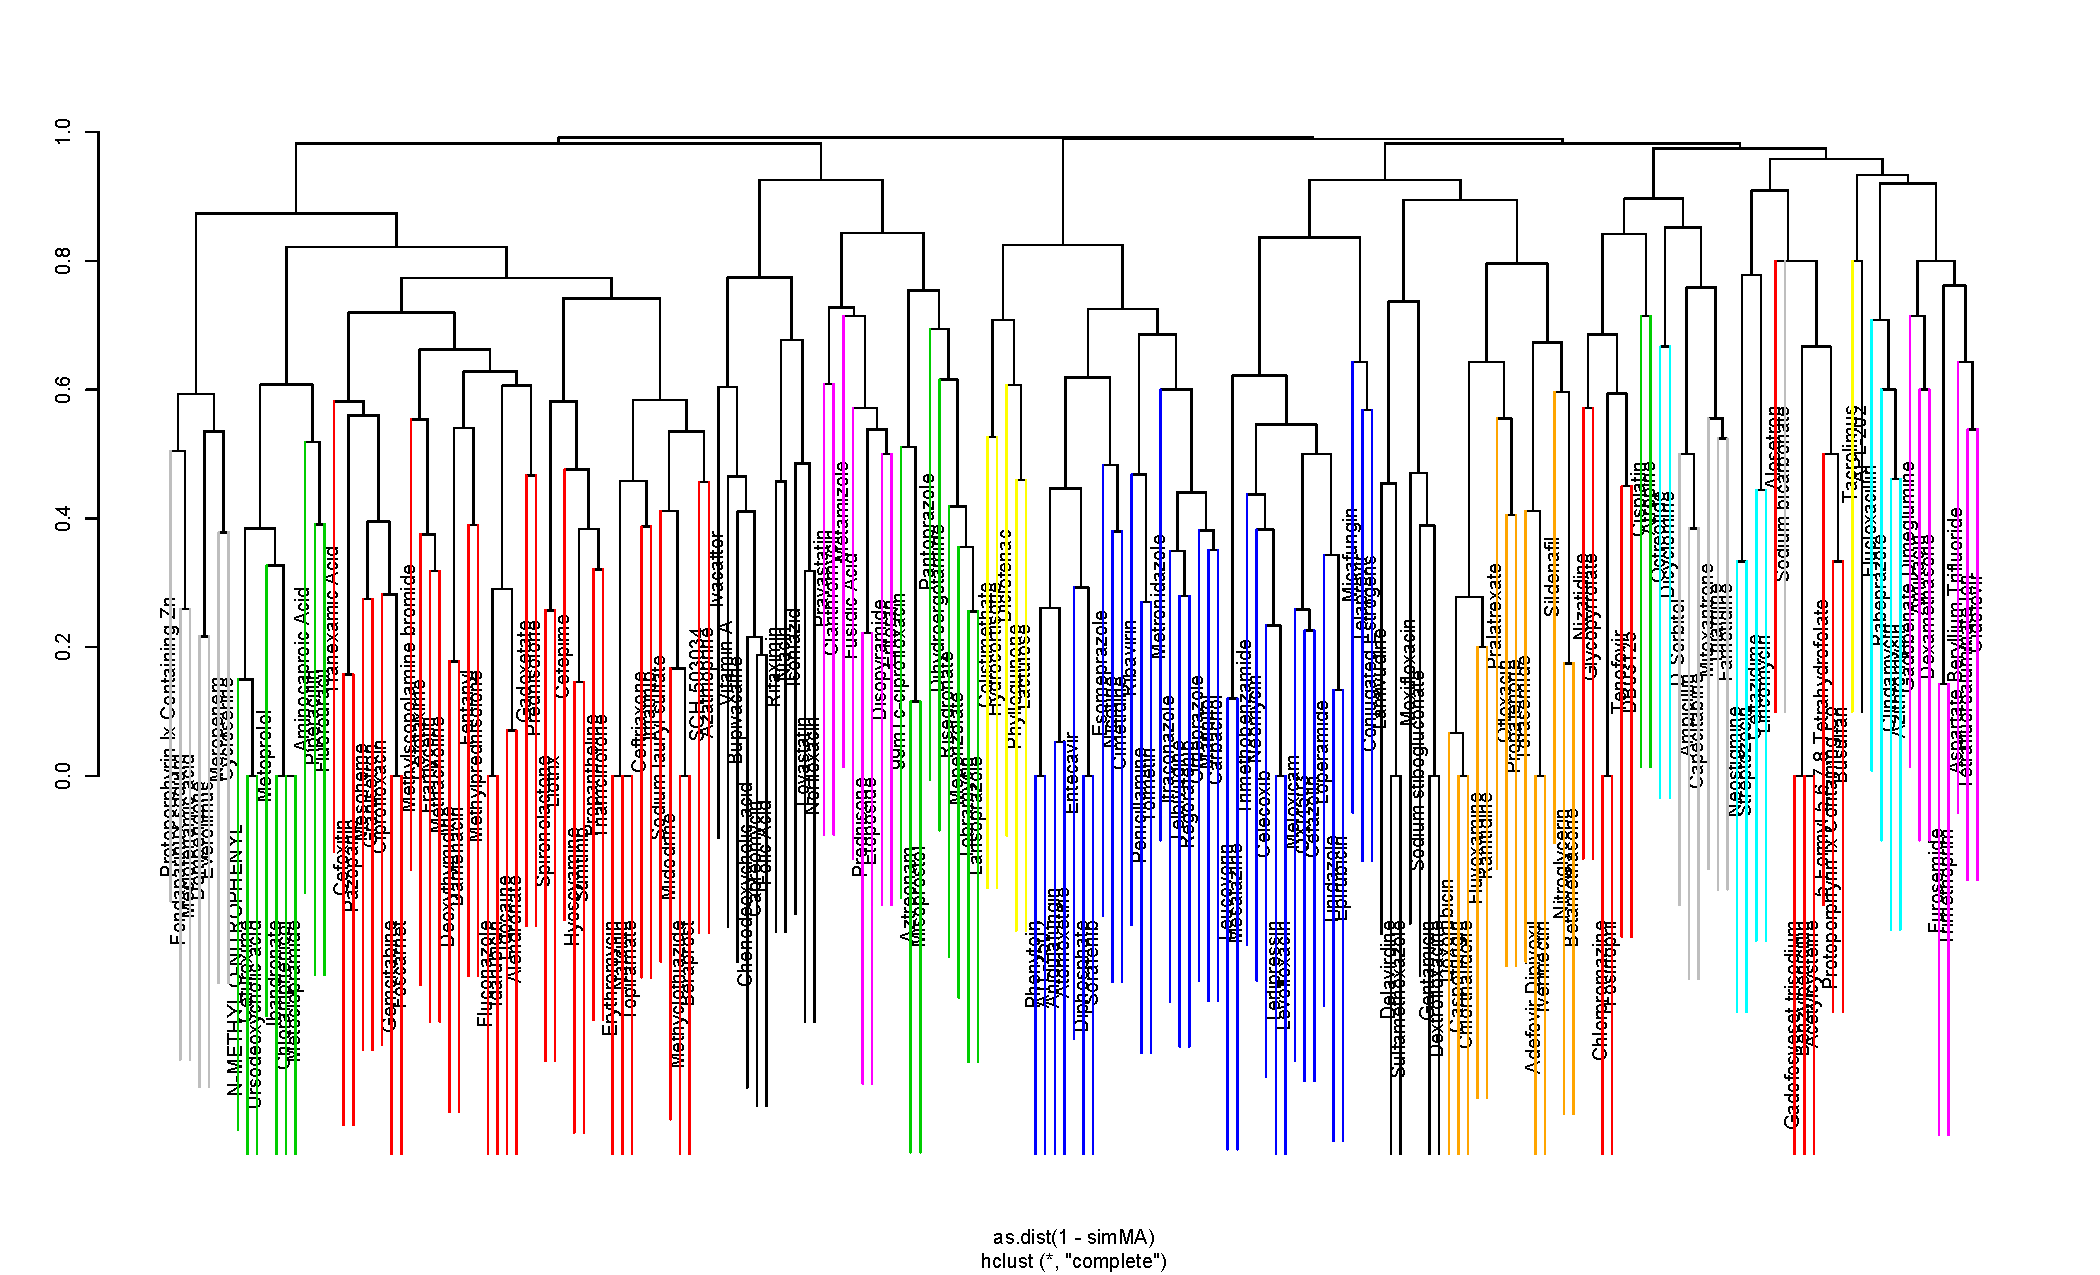
\includegraphics[width=17cm,totalheight=12cm]{/LaTex/DiseaseNets/dendro3.pdf} % OK
  \end{center}
\special{center} \caption{Dendrogram of clusters, based on chemical fingerprint properties of 189 drugs}
\label{dendro2}
\end{figure*}
%%%%%%%%%%%%%%%%%%%%%%%%%%%%%%%%%%%%

In figure \ref{fig:heat} we show the results of applying the Tanimoto similarity score to the available drugs and the resultant heatmap. There are  a small number of well defined clusters along with patches of smaller clusters. The silhouette plot indicates that  values near one (unity) indicates  that the observation is well placed in its cluster; values near zero show that it's likely that an observation should belong to some other cluster. 

\begin{itemize}
\item 0.71-1.0  - A strong structure has been found
\item 0.51-0.70 - A reasonable structure has been found
\item 0.26-0.50 - The structure is weak and could be artificial
\item $<$ 0.25 No substantial structure has been found
\end{itemize}


%%%%%%%%%%%%%%%%%%%%%%%%%%%%%%%%%%%%
\begin{figure}[h]
  \begin{subfigure}[b]{0.3\textwidth}
    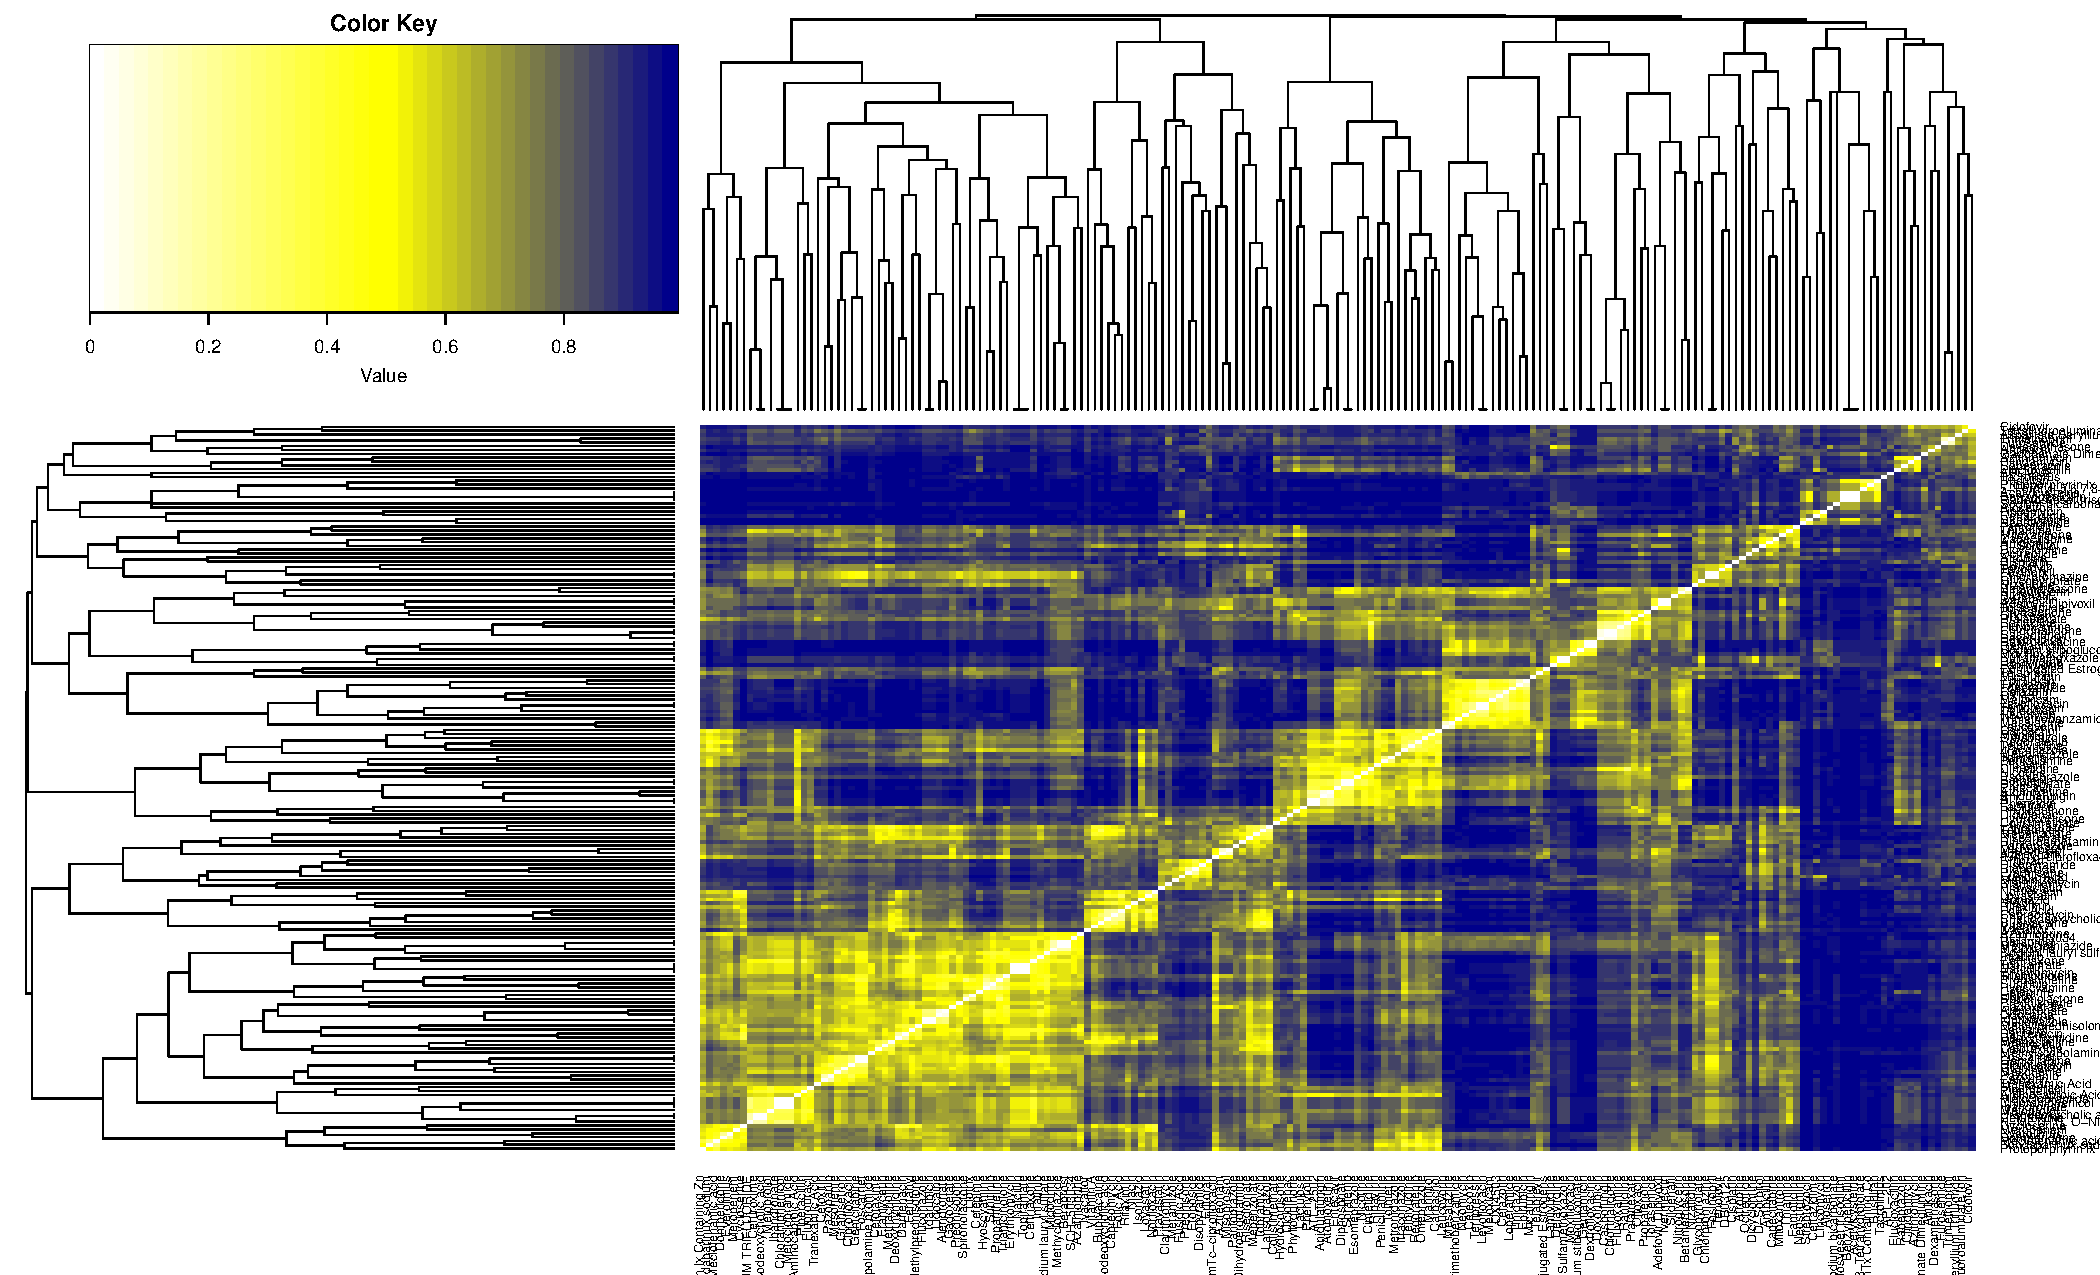
\includegraphics[width=8cm,totalheight=10cm]{/LaTex/DiseaseNets/heat1.pdf} % OK
    \caption{Heatmap of clusters based fingerprint-based Tanimoto similarity matrix}
    \label{fig:heat}
  \end{subfigure}
  \hfill
  \begin{subfigure}[b]{0.5\textwidth}
    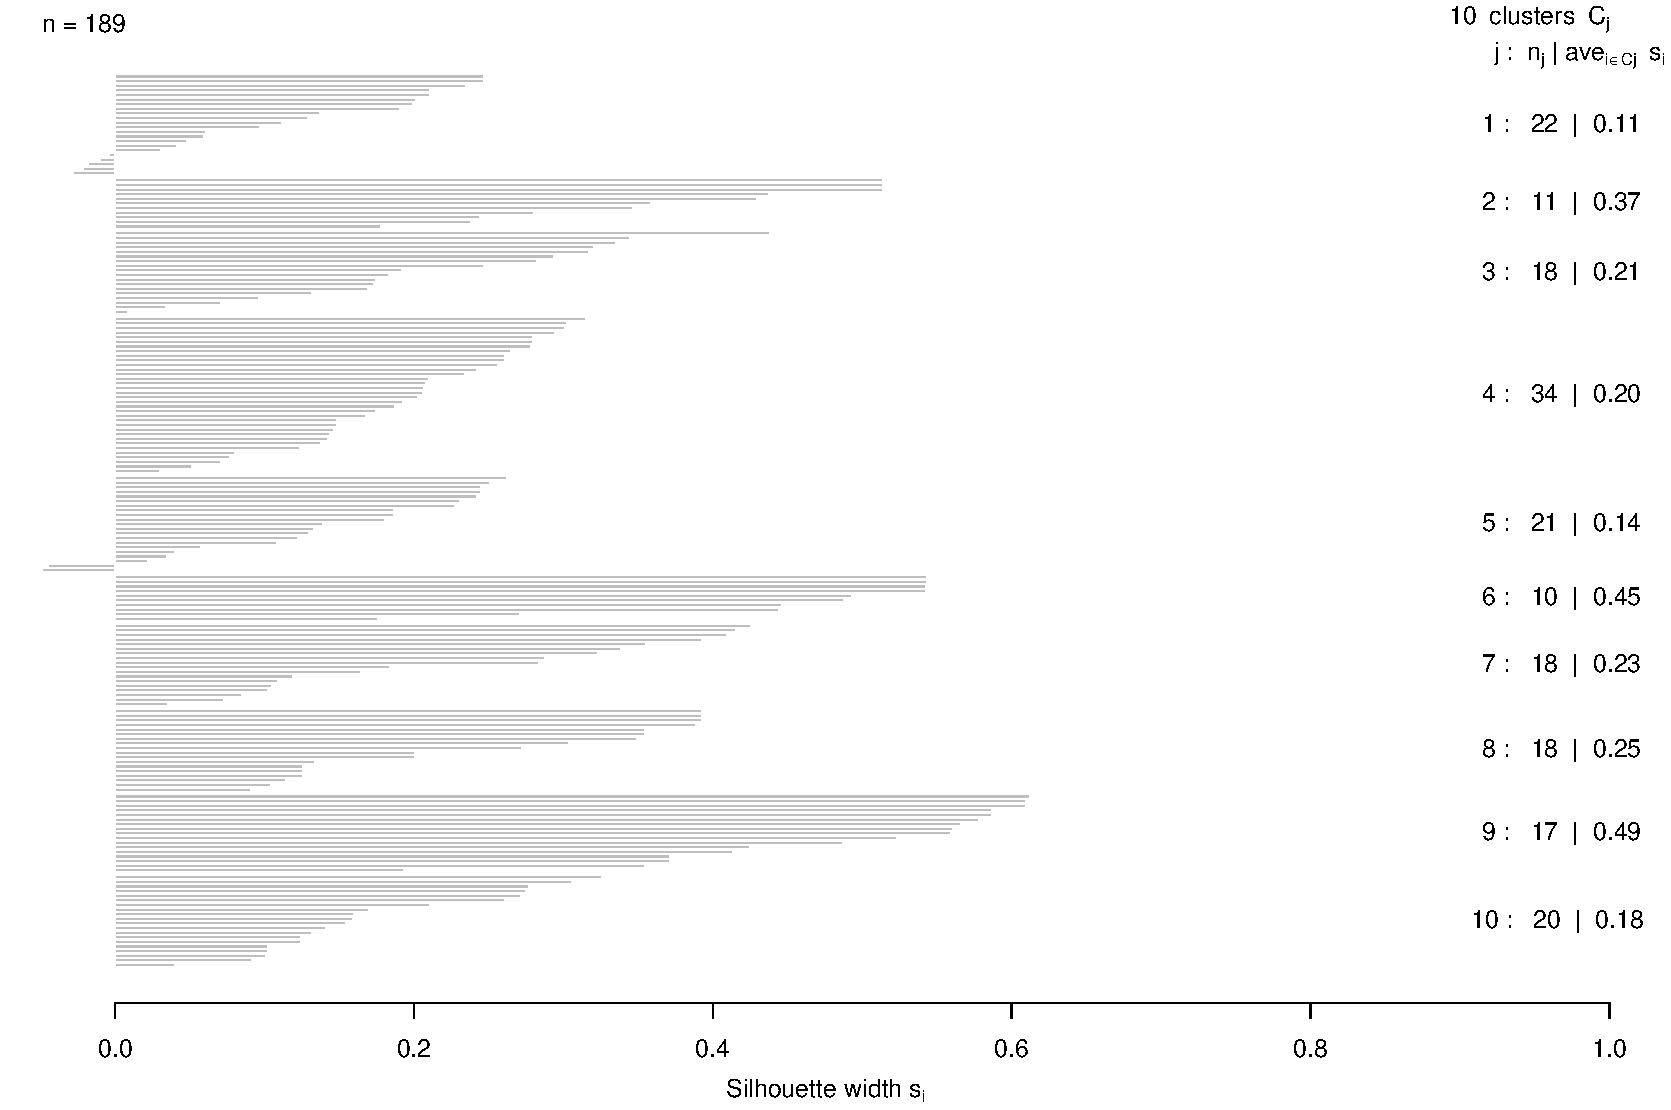
\includegraphics[width=7cm,height=10cm]{/LaTex/DiseaseNets/silhoutte1.pdf} % O
    \caption{Silhouette plot determining goodness of fit of selected clusters.}
    \label{fig:sillo}
  \end{subfigure}
  \caption{Clustering the 189 drugs based on chemical structure similarity, 10 clusters are identified based on the chemical similarity matrix. The silhouette plot indicates goodness of fit, showing a low to moderate cluster fit. }
\end{figure}
%%%%%%%%%%%%%%%%%%%%%%%%%%%%%%%%%

\section{Conclusions}
Nothing so far.

\section{Acknowledgments}
We would like to thank Christoph Glur for helpful discussion regarding his R data.tree package.



\bibliographystyle{elsarticle-harv}
\bibliography{C:/Latex/kenrefs}
\end{document}



